\documentclass[11pt,a4paper]{article}
% \usepackage[brazil]{babel} % carrega portugues brasileiro
\usepackage[utf8]{inputenc}
\usepackage[T1]{fontenc}
\usepackage[top=2cm, bottom=2cm, left=2cm, right=2cm]{geometry} %margens menores!
\usepackage{graphicx} % incluir figuras .eps
\usepackage{tabularx}
\usepackage{color} % colorir texto
\usepackage{indentfirst}
\usepackage{textcomp}
\usepackage[colorlinks=true]{hyperref}
\usepackage{amssymb,amsmath}
\usepackage{float}
% \usepackage{siunitx}
% \usepackage[ampersand]{easylist}

\title{Manual De Uso Del HERMES}

\author{
       \large
        \textsc{Rafael Diniz}
        \mbox{}\\ %
        rafael@rhizomatica.org\\
        \mbox{Rhizomatica} \\ %
%        \normalsize
%        \texttt{Brasília - Brasil}\\
}
\date{\today}


\begin{document}

\maketitle

\begin{abstract}

This is the user manual of the High-Frequency Emergency and Rural Multimedia Exchange System (HERMES) digital telecommunication system. HERMES combines a set of technologies in order to provide telecommunications services over the HF frequency band. Among these technologies are an affordable HF transceiver, a high performance software-defined modem, the Unix-to-Unix Communication Protocol (UUCP) and a set carefully configured user services which are available over a local WiFi network. This manual addresses the basic equipment operation, including the usage of the web-based graphic user interface (GUI) and the email transport system.

\end{abstract}

\newpage

\tableofcontents

\newpage

\tableofcontents

\setlength{\parindent}{0em}
\setlength{\parskip}{1em}

\section{Introduction}

HERMES is a telecommunication system which operates in the High Frequency (HF) band. HERMES allows digital multimedia exchange between the users and stations, including exchange of text, image, audio or any other file type. The system interface to the users is the well known e-mail protocol, which can be managed and accessed thought the system's web interface or through specialized apps, like DeltaChat\footnote{DeltChat, a multi-plataform e-mail messenger: \url{https://delta.chat/} }. HERMES also support peer-to-peer secure messages between the hosts, which works as a bulletin board system (BBS) so that the peers can connect between them.

The system employs a star topology network in which a gateway station connect to all hosts in remote locations. The gateway station routes e-mail and other messages locally or over the Internet. The synchronization between the data to be sent or received from each remote station is asynchronous and orchestrated by the gateway station in a round-robin fashion (one after another, in order).

\begin{figure*}[!ht]
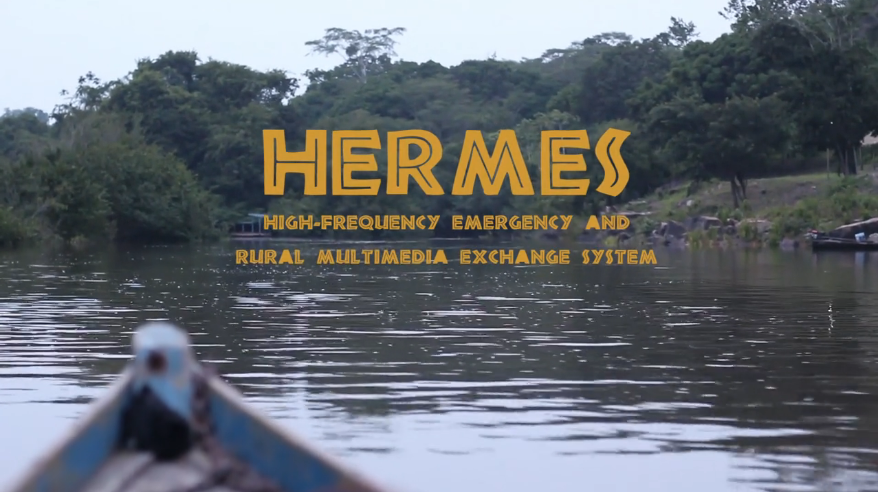
\includegraphics[width=1\textwidth]{pictures/hermes.png}
\end{figure*}

\subsection{HERMES HF Transceiver}

HERMES HF transceiver is typically assembled and delivered together with a WiFi antenna connected to the appropriate connector in the back panel. The front panel of the equipment is shown in Figure~\ref{fig:frontview}.

The HERMES box includes the following input / output interfaces, as shown in Figure~\ref{fig:backview}.

% if there is no explanation of the numbers, it should be itemize and not enumerate

\begin{enumerate}
    \item Back Panel Hermes serial number;
    \item Back Panel Ground connector;
    \item Back Panel Ventilation openings;
    \item Back Panel HF antenna connector (PL-259 / UHF female);
     \item Back Panel Fuse (10A);
     %fuse number
    \item Back Panel 12V DC power input positive (red) and negative (black) terminals;
    \item Back Panel WiFi antenna connector (RP-SMA female);
    \item Back Panel RJ-45 Ethernet port, for connection to external switch or a existing router;
    \item Front Power key (on/off);
    \item Front Panel with 4 indicator LED's (System LED, Antenna Status LED, Connected LED, Tx LED).
\end{enumerate}

\begin{figure}[!ht]
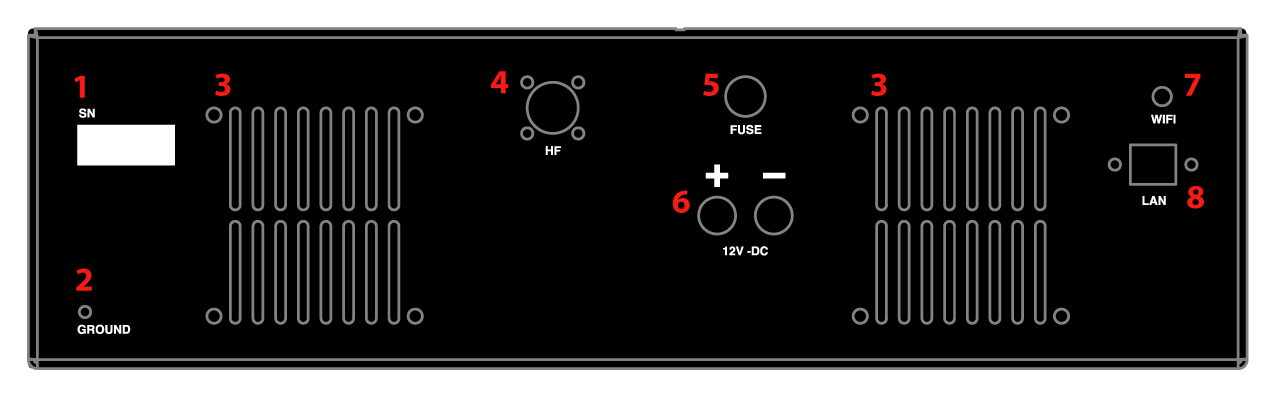
\includegraphics[width=1\textwidth]{pictures/traseiro.png}
\caption{Back view of HERMES box}
\label{fig:backview}
\end{figure}

\begin{figure}[!ht]
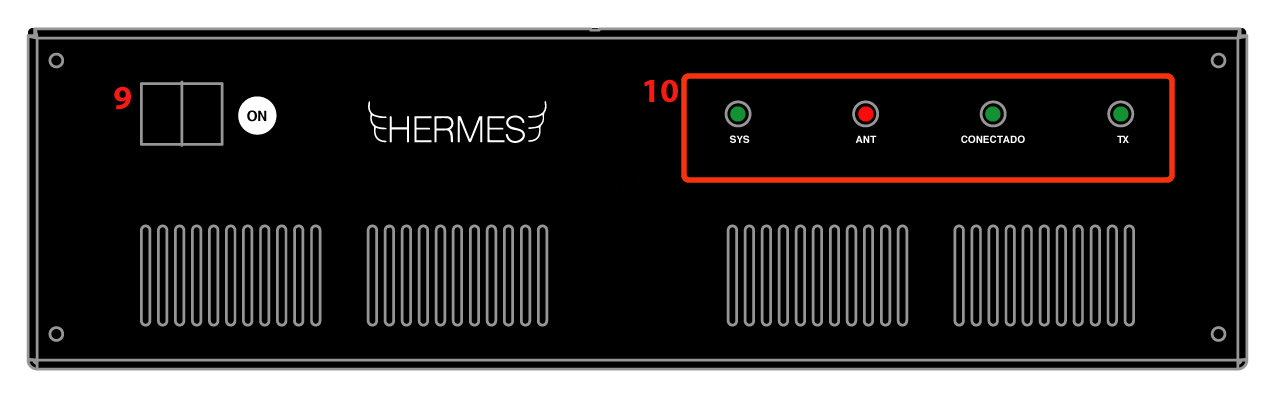
\includegraphics[width=1\textwidth]{pictures/front.png}
\caption{Indicator's LED on front panel}
\label{fig:frontview}
\end{figure}

\subsection{HF Antenna Recommendation}

An HF antenna tuned to the desired operating frequency should be connected to the equipment. Never turn on the equipment without connecting to the HF antenna!

There exist many HF antennas, each one fitting a different purpose. For short and medium range communications (up to about 800 km), a quarter wavelength dipole installed in inverted V configuration is a good and affordable option.

\subsection{Power Requirements}

The system is designed to operate with 12V DC power, but up to 14V the system will work as expected without any problem. A typical setup would use 12V DC from battery power connected to solar controller and panels. Other setup is using a 12V or 13.8V AC/DC power supply. The red connector should be connected to the positive polarity, while the black connector to the negative polarity. The system has polarity inversion protection, but care should be taken to proper power installation of power connections. The equipment consumes approximately 2A in receive mode, and 6A in transmit mode.

\section{Web Interface}

HERMES provides a web interface which can be accessible through a local WiFi network. When accessing HERMES WiFi network, the following information applies:
\begin{itemize}
    \item Network Name (ESSID): HERMES
    \item Password: amazonia
\end{itemize}

Be aware that in some mobile phones a browser will automatically open with the the main HERMES web page, while in others, to access the HERMES web interface you must open the browser and access \url{http://ac1.hermes.radio} or \url{http://10.0.0.1}.

   \begin{figure}[!ht]
    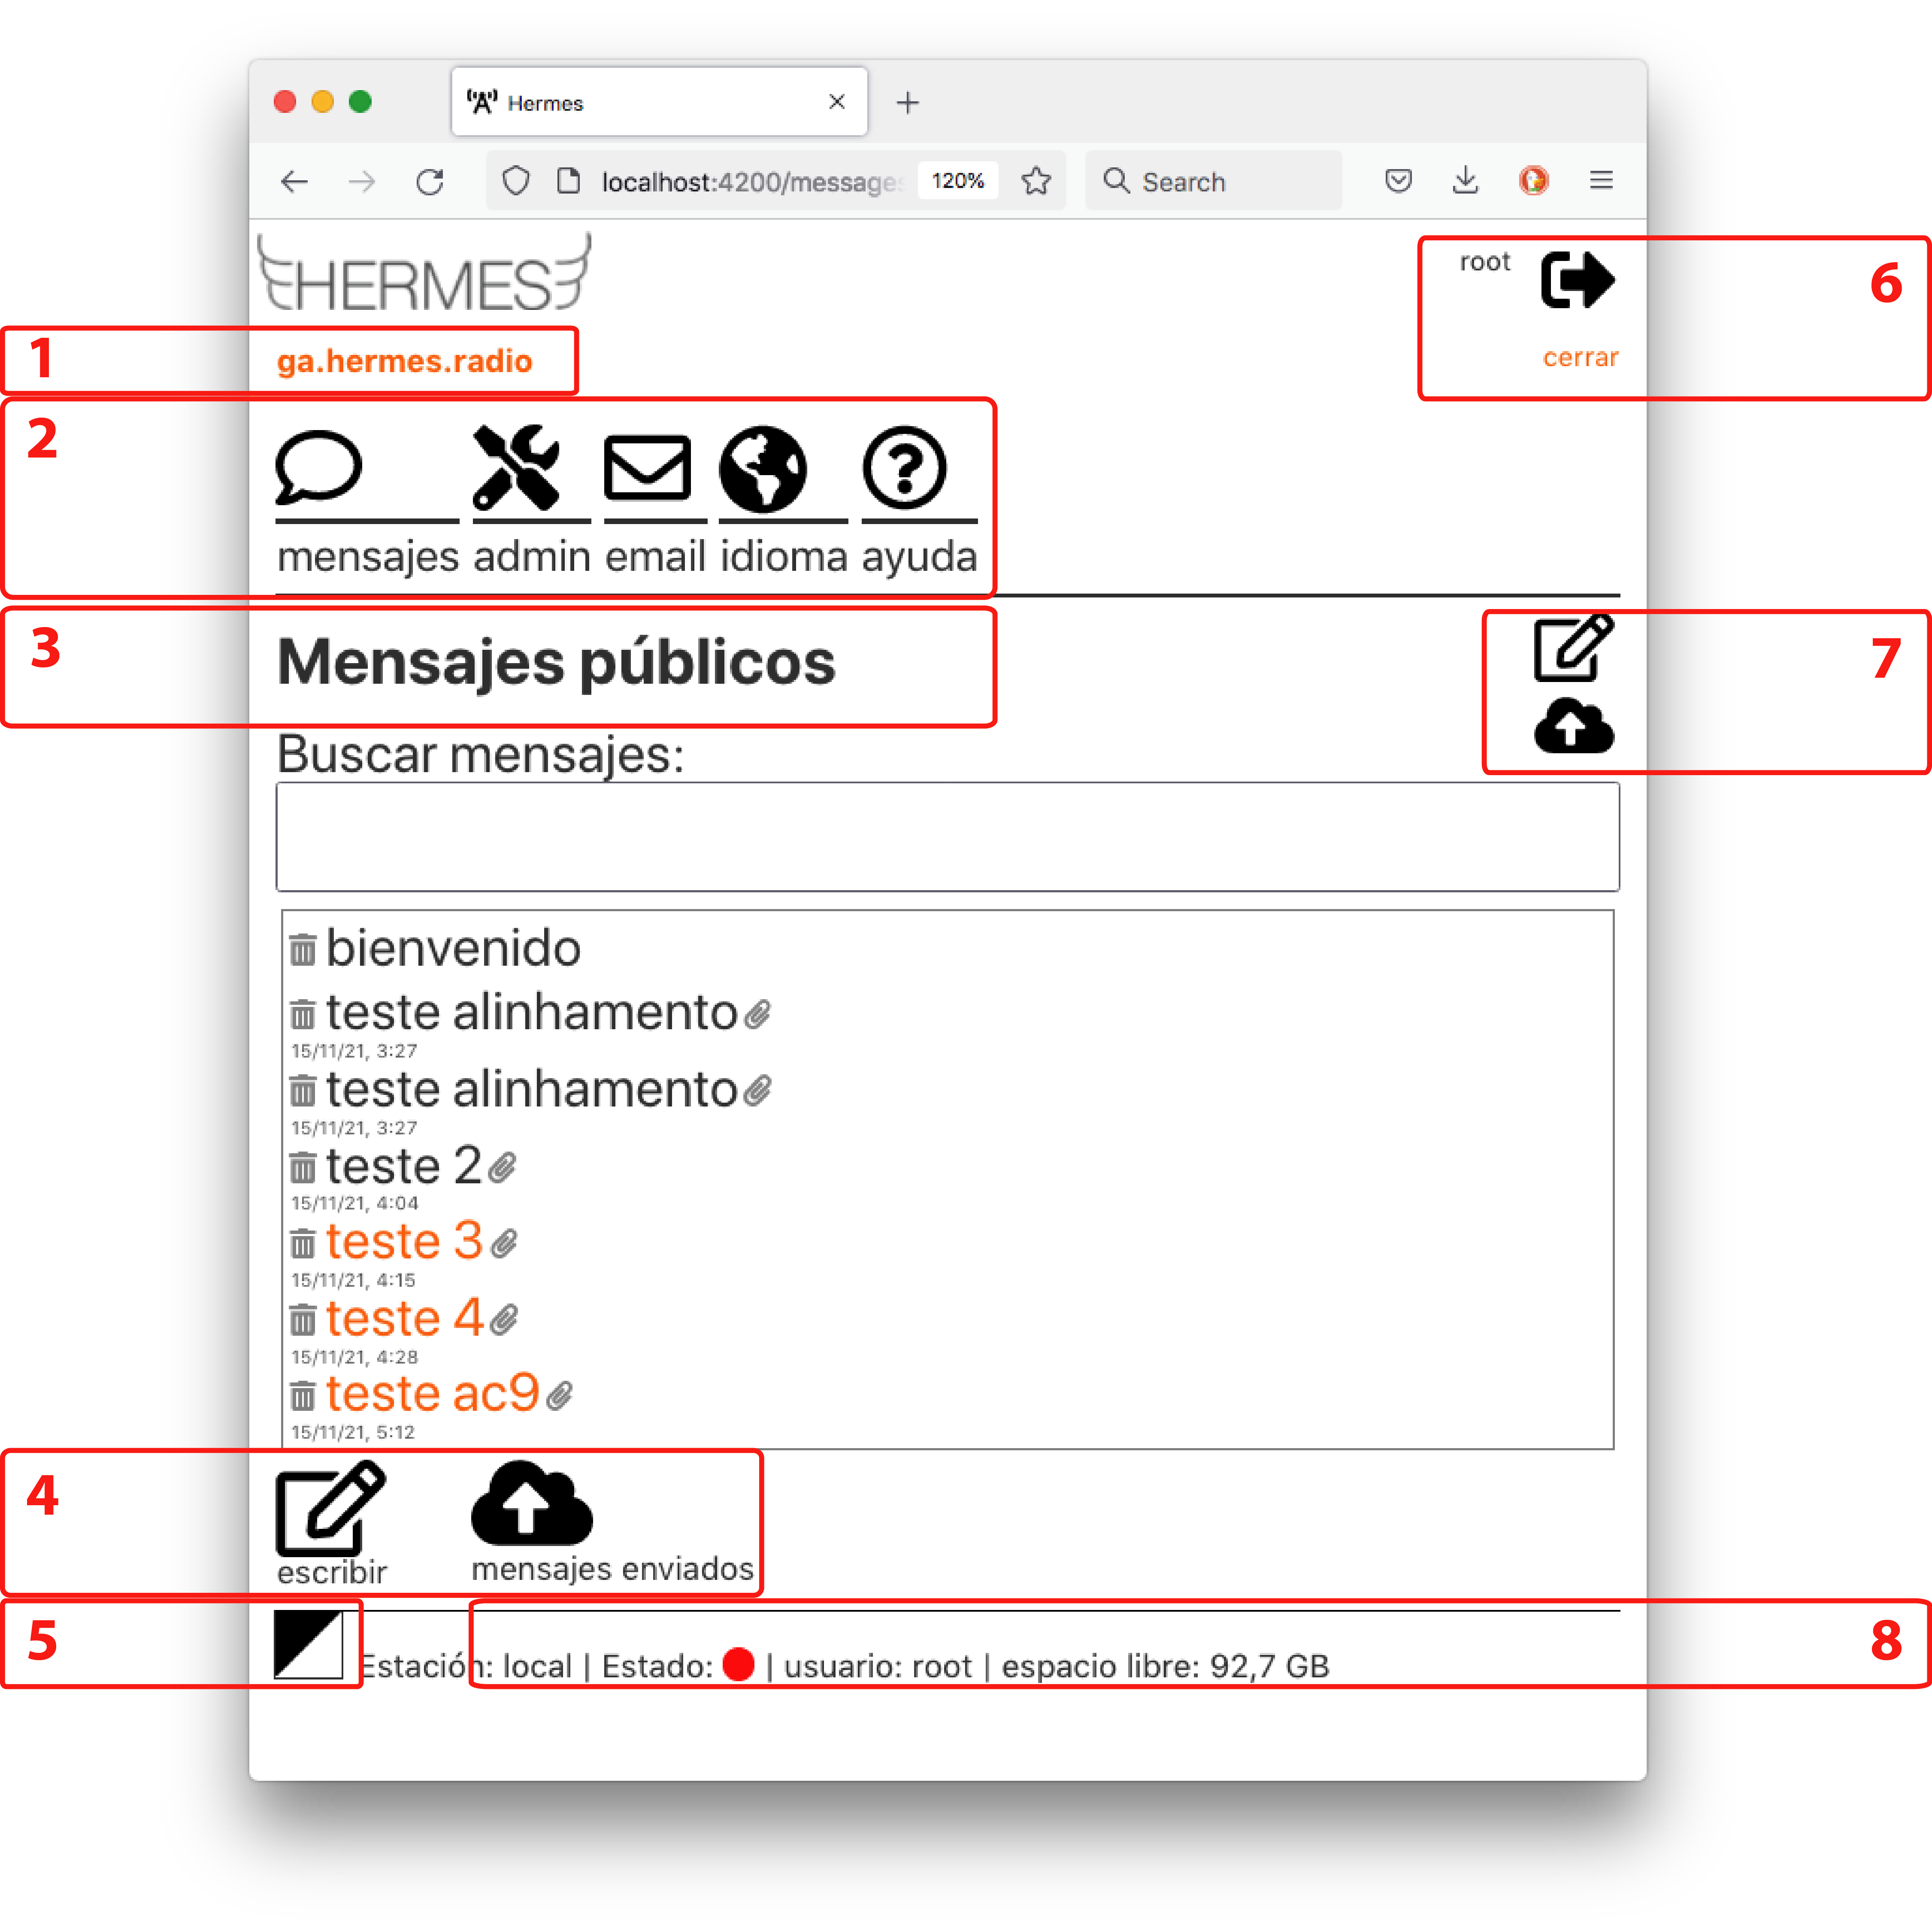
\includegraphics[width=1\columnwidth]{pictures/interface-es.png}
    \caption{Hermes Home page and elements}
    \label{fig:interface}
    \end{figure}
    
On the main page \ref{fig:interface} you will find the following links:

\begin{enumerate}
    \item Domain name of your current station
    \item Main menu;
    \item Page title;
    \item Compose and sent messages link;
     \item Login and logout link and info;
     \item Dark mode activator tab;
    \item Compose and sent messages shortcut;
    \item Station information and status;
\end{enumerate}
    
    The web interface allows users to manage e-mail accounts, to perform radio configurations (like setting frequency and SSB mode) and exchange direct messages between stations (BBS). The interface also contains its own administrative section, for managing users which can access HERMES administrative web interface. Important to note that same user name created for using the administrative interface will be used for the e-mail, for example, user "amelia" in the local interface will have the email "amelia@ac2.hermes.radio", the station that corresponds to the internet domain name, in this example, it'll be "ac2.hermes.radio". Each station domain name is written in the header on the Hermes web interface.

\subsection{Administrative Interface}
\label{admininterface}

\begin{figure}[H]
    \centering
    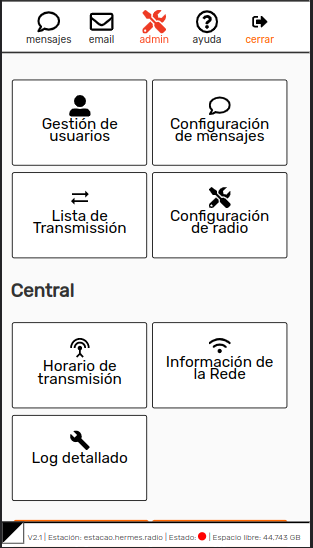
\includegraphics[width=0.5\columnwidth]{screenshots/frontend/es/admin.png}
    \caption{Admin interface}
    \label{fig:admin}
\end{figure}

To access admin features, you need an admin password. While anyone can create an user account, only the system's admins can create new administrator users and give admin power to other users. To login, click on the login icon on the top right of the web interface. The default administrator login username is "root" and password "caduceu".

Inside the administration section, an admin user will find the following options: users management, messages administration, network information, stations, detailed log and radio configuration. If the station is the central station it will also find the central station menu.

\subsubsection{Users management} 

Allows creation of new users, updating data of registered users and to delete users of the system. Every username correspond to an email account with the same name of the kind username@servername. On this station the server name will be shown in orange below the Hermes logo.
    
    \begin{figure}[H]
    \centering
    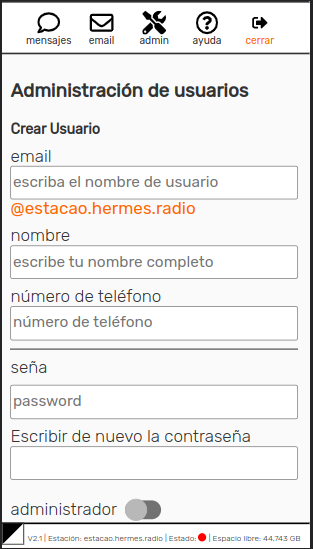
\includegraphics[width=0.5\columnwidth]{screenshots/frontend/es/createuser.png}
    \caption{Create user interface}
    \label{fig:createuser}
    \end{figure}
    
    Administrators can also give admin powers to regular users, by clicking on the "is admin" checkbox on the update user interface.

\subsubsection{Messages administration}  
\label{gui_msg_admin}

On this link, the admin can determine who will be able to attach files on public messages between stations: everyone; only registered users or only administrators
   
    \begin{figure}[H]
    \centering
    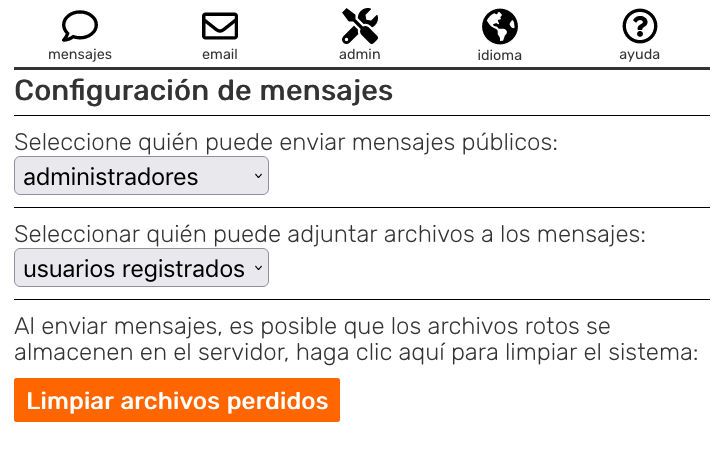
\includegraphics[width=0.5\columnwidth]{screenshots/frontend/es/messageadm.png}
    \caption{Messages administration Interface}
    \label{fig:messageadm}
   
    \end{figure}
    
\subsubsection{Network info} 
\label{gui_net_info}

Displays some information about the system, such as network addresses, callsign, servername etc
     \begin{figure}[H]
     \vspace{-10pt}
    \centering
    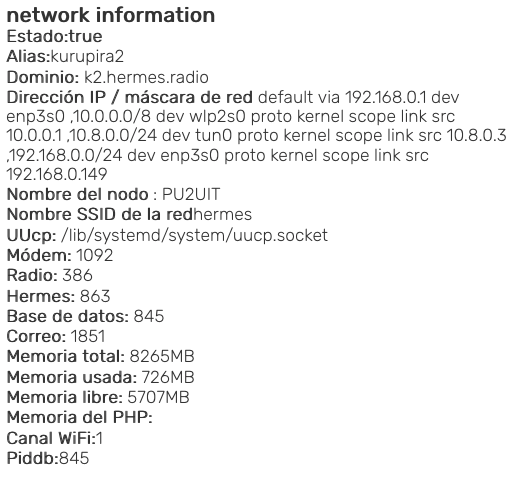
\includegraphics[width=0.5\columnwidth]{screenshots/frontend/es/networkinfo.png}
    \caption{Network information page}
    \label{fig:netinfo}
  
    \end{figure}

\subsubsection{Stations} 

% TODO: This is certainly not correct... 
Provides a list of the available stations on the system.
    
\subsubsection{Detailed Log}
Provides access to system logs, such as email logs and UUCP logs, that register every activity on the system.
    
    \begin{figure}[H]
    \centering
    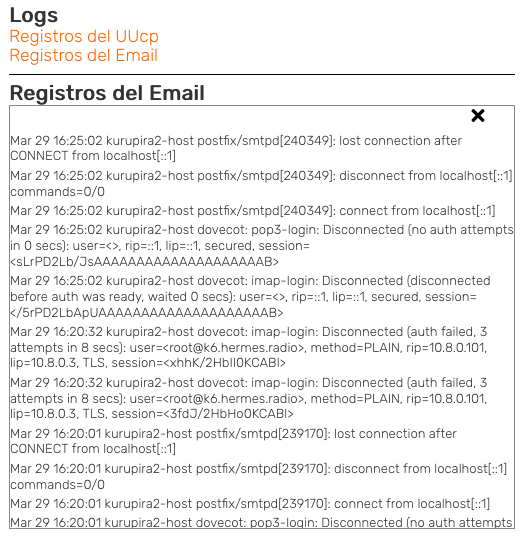
\includegraphics[width=0.5\columnwidth]{screenshots/frontend/es/logs.png}
    \caption{Logs page on the web interface}
    \label{fig:logs}
\end{figure}

\subsubsection{Radio configuration}

Provides a direct interface to  change some radio settings like frequency, transmission mode, restore factory configuration and it also allows to view some sensors readings about the HF antenna of the system. 

\begin{figure}[H]
    \centering
    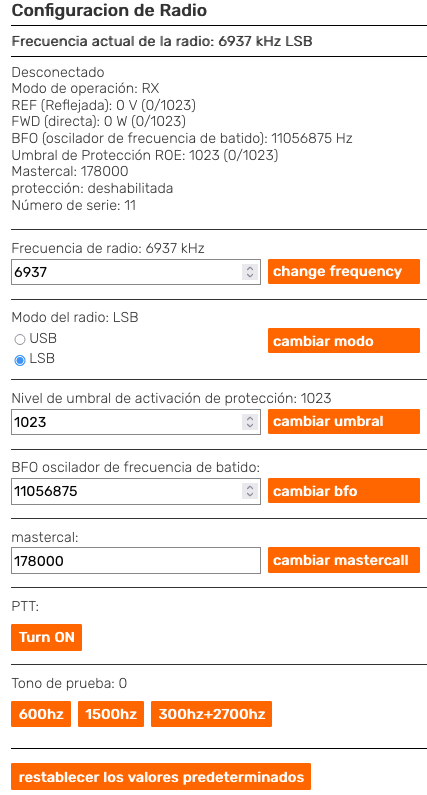
\includegraphics[width=0.5\textwidth]{screenshots/frontend/es/radioconfig.png}
    \caption{Radio configuration interface}
	\vspace{-10pt}
    \label{fig:radioconf}
\end{figure}

\subsection{Public Messages  (BBS)}

Direct messages can be sent between stations with support for cryptography and  multimedia compression. These messages can be found in the main page of the web interface.

\subsubsection{How to write public messages}


\begin{figure}[H]
    \centering
    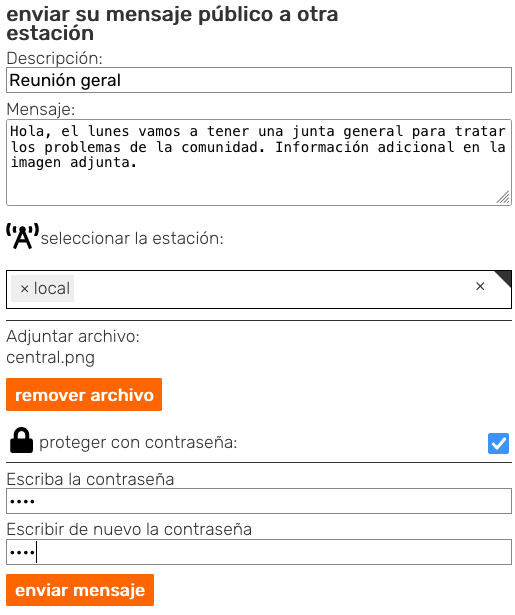
\includegraphics[width=0.5\textwidth]{screenshots/frontend/es/publicas.png}
    \caption{Interface to compose messages}
    \label{fig:compose}
\end{figure}

\begin{figure}[H]
    \centering
    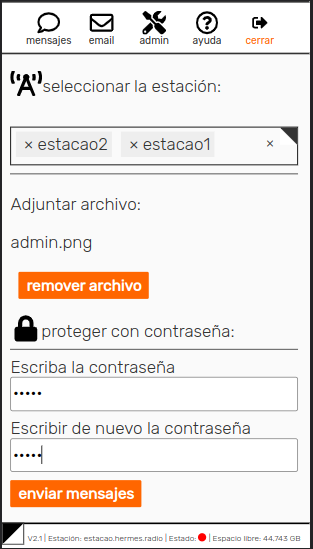
\includegraphics[width=0.5\textwidth]{screenshots/frontend/es/publicas2.png}
    \caption{Interface to compose messages}
    \label{fig:compose2}
\end{figure}

By clicking on the compose (
\includegraphics[height=0.8\baselineskip]{pictures/edit.png})icon, it's possible to write a new message and to attach files such as images or audio files. The system's admin can determine who can attach files to public messages. 

Public messages can be sent to your own station, which is an easy way to publicize news inside your own community.

Public messages can also be password protected, which means that only the ones that know the password will be able to read their content, but their description still will be readable by everyone. Have in mind that once a password for the message (has to be at least 4 characters) is defined, there is no way to recover it, nor to change it.

On the message administration link on the admin session, a system administrator can change who can attach files on messages between stations: everyone with access to the network, only registered users, or only administrators.

Because the radio propagation of data is very low, file attachments are constrained to 20KB sizes. The system will accept inputs for image and sound up to 30 MB and for other files up to 2 MB, and will try to compress them to fit the maximum size for packages. For image and sound, the resolution can be changed, and the quality may be affected. For other formats, a simple compressor will be applied, and message packages with size greater than 20 KB will be cancelled.

\subsection{Transmission Queue}

All the data exchange in the HERMES system is done through UUCP. As an asynchronous protocol, 
all the data is first queue before being transmitted. The elements of the UUCP queue are called "jobs", and each job in the HERMES system can be an e-mail, a public message, or special remote command execution message (for example, to inform of a new e-mail user creation). A system administrator can cancel a job before it is sent. Administrators can also erase the public messages for any reason, including the case when the equipment storage space is reaching its end. The storage space available is shown on the web interface footer.

The queues of all stations are transmitted from times to times, when the gateway station connects to each remote station. In an emergency case, the system administrator can force message transmission queue by clicking on the "transmit now" link. This can interrupt receiving messages from other stations for a while and should be avoided unless it's really necessary.

\subsection{Languages supported}
\label{langs}

This version of the Hermes system is translated to Portuguese and Spanish, and the versions can be accessed on the languages tab of the main menu

\begin{figure}[H]
    \centering
    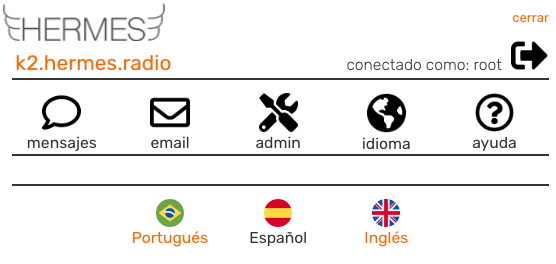
\includegraphics[width=0.5\textwidth]{screenshots/frontend/es/languages.png}
    \caption{Page to access translations}
	\vspace{-10pt}
    \label{fig:languages}
\end{figure}


\section{E-mail}
\label{email}

\begin{figure}[H]
  \centering
  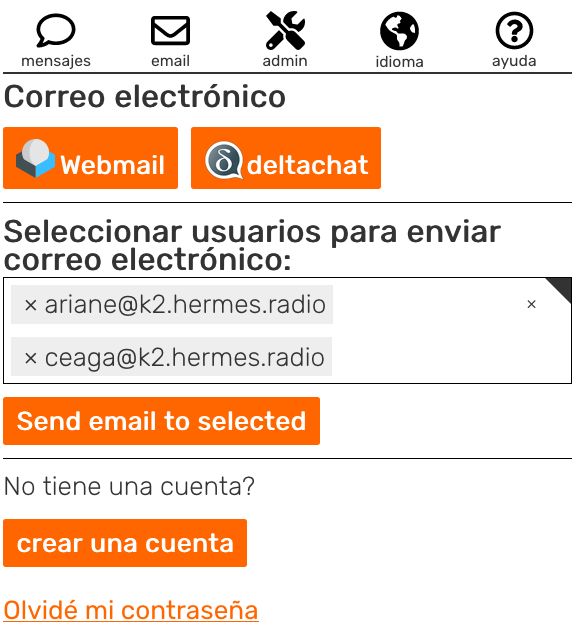
\includegraphics[width=0.5\columnwidth]{screenshots/frontend/es/email.png}
  \caption{Page to access webmail interface}
  \vspace{-10pt}
  \label{fig:webmail2}
\end{figure}

The main service provided by the HERMES system is the electronic mail (E-mail). E-mail is communication protocol which attributes to each e-mail bearer an address in the format "username@host". The "username" part of the email is created by a HERMES administrator user in the web interface, while the host (also called domain) is already set in the system, and typically has the format "community\_id.hermes.radio". So a typical HERMES emails looks like, for example, "amelia@ac4.hermes.radio". The "username" is the same username as created in the user creation page in the HERMES administration interface.

HERMES email users can send and receive e-mail just like any other e-mail user. The only restriction which must be considered is that telecommunication in HF is slow, so emails with large attachments will be cancelled by the system, with the appropriate cancellation message sent to the user.

While there are many e-mail clients, like Thunderbird and Outlook Express, the recommended e-mail client to be used with HERMES is DeltaChat. DeltaChat Android, Windows, MacOS and Linux installer is available for download through the interface, while as a backup option, RoundCube webmail client is also accessible through HERMES web interface.


\subsection{DeltaChat}

\begin{figure}[H]
    \centering
    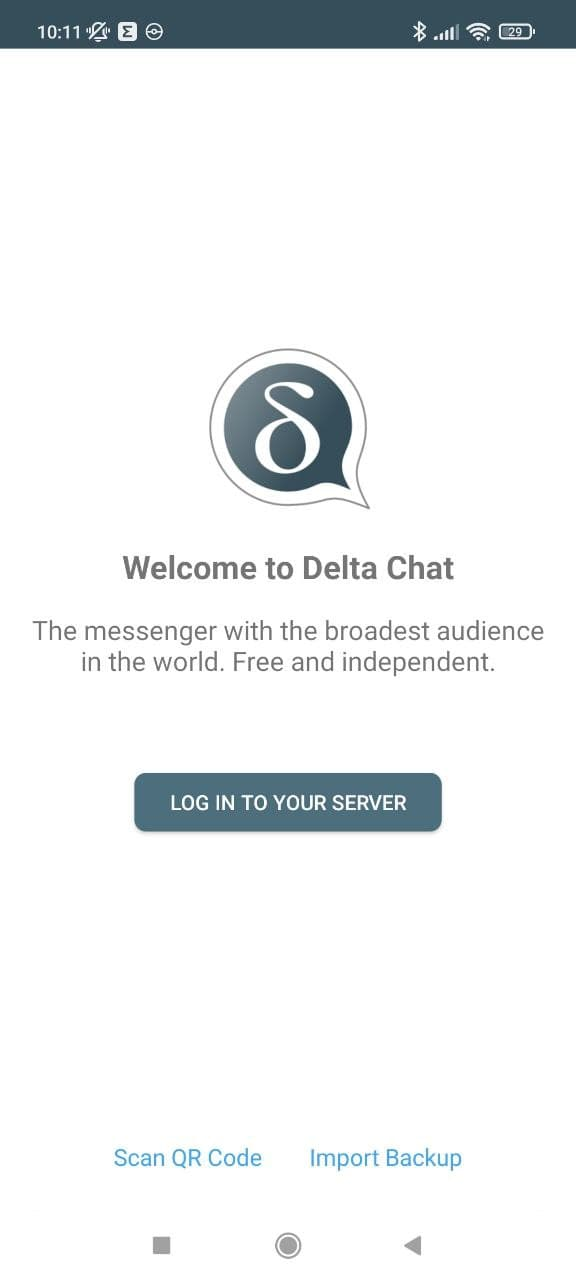
\includegraphics[width=0.3\columnwidth]{screenshots/deltachat/en/intro.jpg}
    	\caption{Deltachat intro (first screen)}
	\vspace{-10pt}
    \label{fig:deltachat-intro}
\end{figure}

\begin{figure}[H]
    \centering
    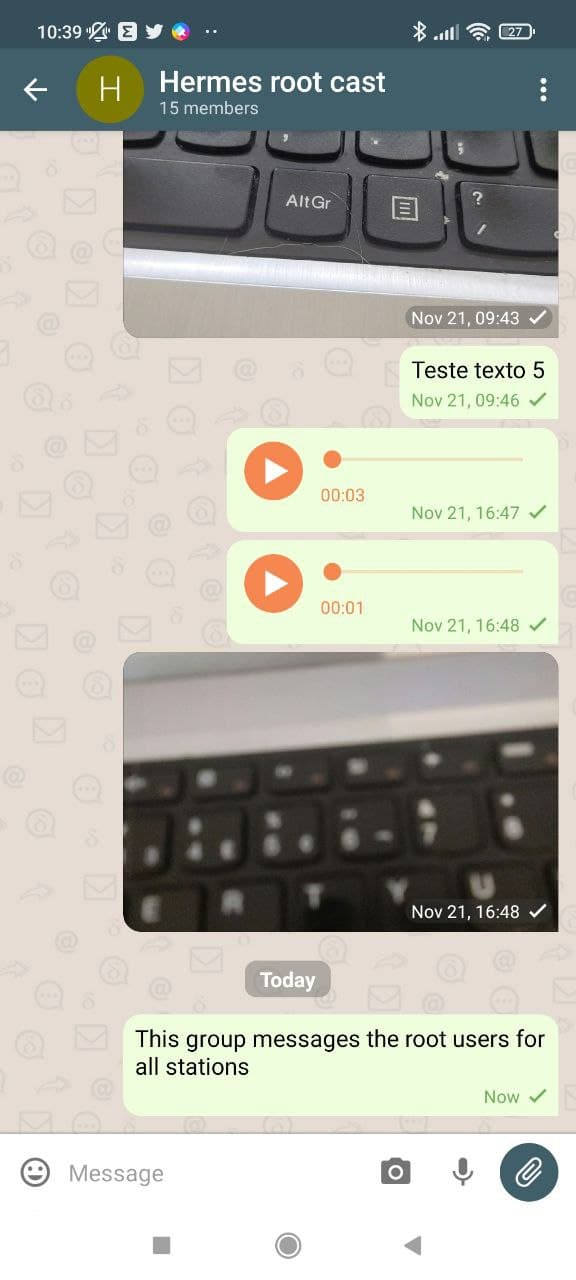
\includegraphics[width=0.3\columnwidth]{screenshots/deltachat/en/chatroom.jpg}
    	\caption{Deltachat chat room example}
	\vspace{-10pt}
    \label{fig:deltachat-chatroom}
\end{figure}

With the Deltachat application, you can use HERMES emails to carry out personal communications for exchanging messages; This app works on most common smartphones and feels like a common message application such as whatsapp or telegram. Keep in mind that due to the message transmission schedule, messages may take a while to arrive, depending on the amount of messages in the queue and the opening hours of the transmitters.

\subsubsection{Installation}

The Deltachat is available in the most common app stores, but if you're not connected directly to the internet, you can download it through the HERMES web interface, selecting one of the packages provided according to your device operational system. We provide installation files for Android, GNU/Linux, Windows and MacOSX mobile or computer systems. and can be accessed here if you're reading this using a HERMES system network: \href{ http://10.0.0.1/dowloads/deltachat.apk}{Android},  \href{ http://10.0.0.1/dowloads/deltachat.exe}{Windows},  \href{ http://10.0.0.1/dowloads/deltachat.deb}{Debian} and \href{http://10.0.0.1/dowloads/deltachat.dmg}{Mac OS}

% FEITO qual endpoint do frontend?

\subsubsection{Configuration}

The HERMES system includes an encryption system suitable to fit multimedia messages like images or audio and send them by HF.  End-to-end encryption should be disabled in order to the server-based image and audio compression work, otherwise image and audio exchange will not be possible.
The steps to find this feature in Deltachat is: Burger Menu (
\includegraphics[height=0.78\baselineskip]{pictures/burger.png}) -> Settings -> Advanced -> Autocrypt, turn off: Prefer End-To-End Encryption) as shown in Figure~\ref{fig:deltachat-adv_p2pe}.

\begin{figure}[H]
    \centering
    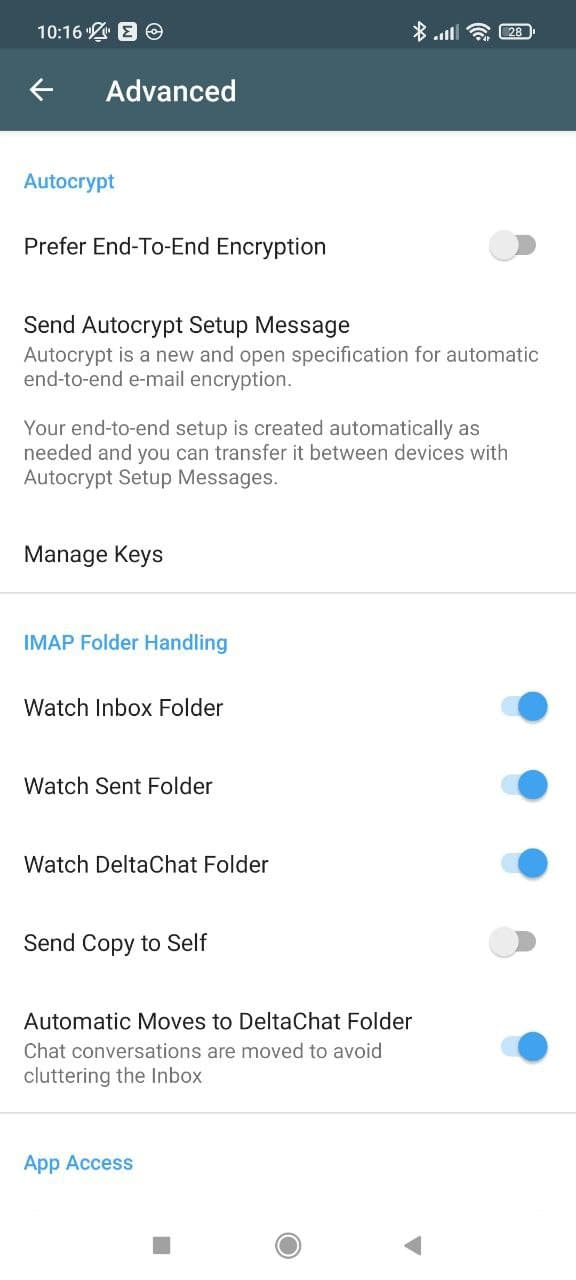
\includegraphics[width=0.3\columnwidth]{screenshots/deltachat/en/adv_p2pe.jpg}
    	\caption{Deltachat Advanced settings}
	\vspace{-10pt}
    \label{fig:deltachat-adv_p2pe}
\end{figure}

The Deltachat by default, tags its emails and show only the "known" messages (emails) that was sent by another Deltachat application. In order to be able to interact with e-mails from any e-mail client software, enable the option "show all emails".
The steps to find this feature in Deltachat is:  Burger Menu (
\includegraphics[height=0.78\baselineskip]{pictures/burger.png}) -> Settings -> Chats and Media -> Show Classic E-Mails -> All. As shown in Figure~\ref{fig:deltachat-allemails}

\begin{figure}[H]
    \centering

    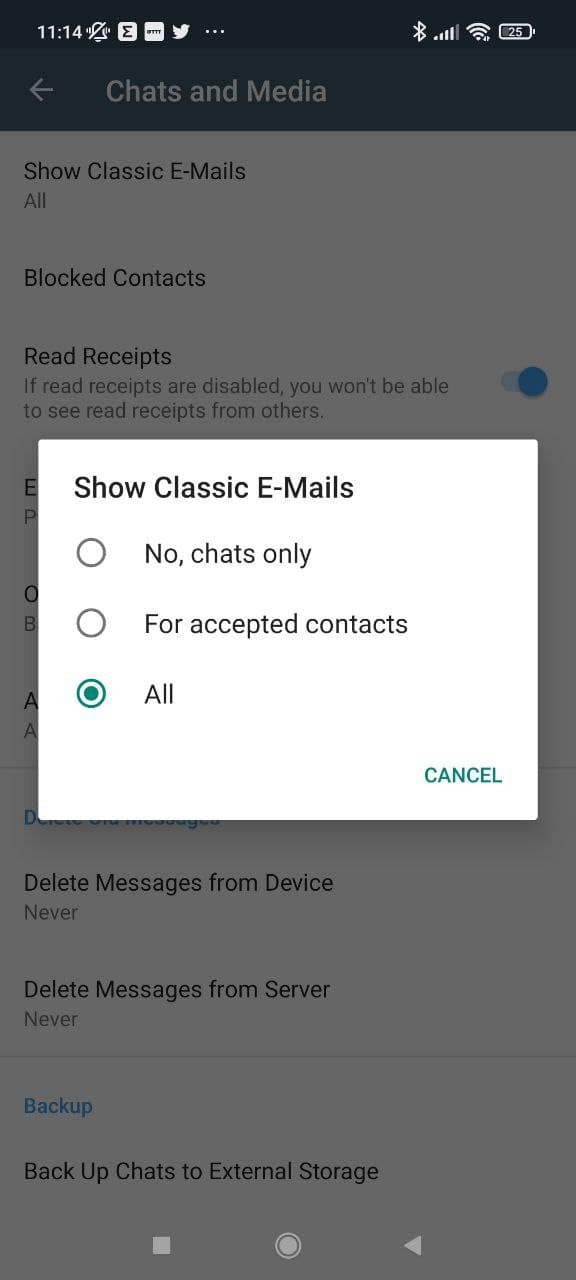
\includegraphics[width=0.3\columnwidth]{screenshots/deltachat/en/allemails.jpg}
    	\caption{Deltachat Setup all emails}
	\vspace{-10pt}
    \label{fig:deltachat-allemails}
\end{figure}

\subsubsection{Usage}

In order to configure the DeltaChat e-mail client, first an e-mail account should be created, as described in section~\ref{admininterface}. In order to login to an e-mail account, just the e-mail address and password fields should be filled, as shown in Figure~\ref{fig:deltachat-login}.

\begin{figure}[H]
    \centering
    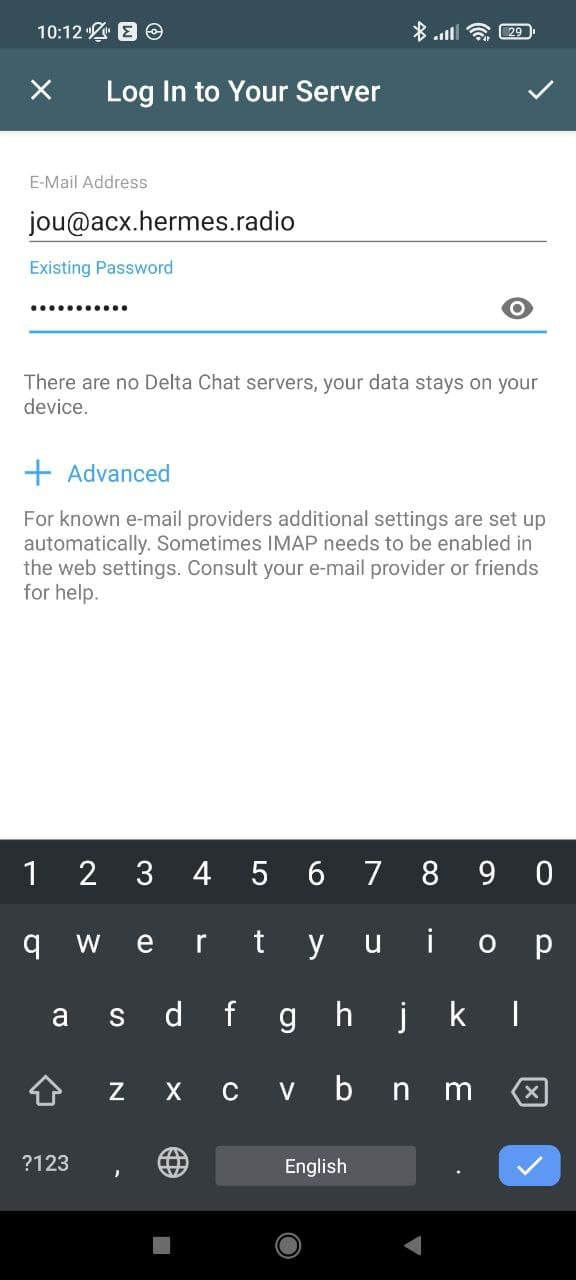
\includegraphics[width=0.3\columnwidth]{screenshots/deltachat/en/login.jpg}
    	\caption{Deltachat Login example}
	\vspace{-10pt}
    \label{fig:deltachat-login}
\end{figure}

% TODO: put DC pictures here
\subsection{Other email clients}
Other email clients can also be used. We can't cover all cases, but the HERMES setup uses default services like IMAP to synchronize email folders and SMTP to send the messages, the specifics technical information about the ports can be found in the appendix: \ref{apx_net_email}

\section{Troubleshooting}

In case of problem in the Antenna, a red led in the antenna (ANT) position will light up on the HERMES box, in this case, check the correct position of the power supply wires and check the position and integrity of the Antenna, coaxial cable, and the transmitter.

If the messages in the transmission list are not being transmitted over time, check if the radio settings have been changed, if that's not the case, it's possible that the other stations are offline.
%To remedy you could restore the factory default settings.

The HERMES web interface also indicates when something is wrong with the system. When a red dot appears on the footer bar (figure \ref{fig:status}), it becomes interactive, and when clicked, it lists the names of the services that can have a problem.

\begin{figure}[H]
    \centering
    
\includegraphics[width=0.8\columnwidth]{screenshots/frontend/es/status.png}
    	\caption{Red dot on the web interface can be clicked to check what part of the system may be broken}
    \label{fig:status}
\end{figure}


\pagebreak
\appendix{techinfo}
\label{techinfo}
\section{Appendix - technical information}
\subsection{Network Information}
\label{apx_net_info}

Each HERMES system is a WiFi access point. The configuration is:
\begin{itemize}
\item WiFi Network Name: \texttt{HERMES}
\item WiFi Password: \texttt{amazonia}
\end{itemize}

The IP of the HERMES station (in the wireless interface) \textbf{10.0.0.1} and the ethernet connection will connect as a dhcp client in a already existing network. 

%\item Server address: \url{hermes.radio} (IP \url{10.0.0.1})
\subsection{Network Services} 
\label{apx_net_services}

\subsubsection{E-mail services}
\label{apx_net_email}

The email system provides these public services. The email settings are the following:

\begin{itemize}
    \item Server address: \url{hermes} (IP \url{10.0.0.1})
    \item SMTP (Simple Mail Transfer Protocol): port \texttt{25}
    \item SMTPS (Secure Simple Mail Transfer Protocol): port \texttt{465}, with SSL support 
    (used for deltachat, the certificates valid until 2031)
    \item IMAP (Internet Message Access Protocol): port \texttt{143}
    \item Webmail URL acessible: \url{http://hermes/mail} or \url{http://10.0.0.1/mail}
\end{itemize}

The use of these settings should not be needed by the user, as DeltaChat automatically identify all the settings by entering just the e-mail address and password in the login prompt.

\subsubsection{Web services}
\label{apx_net_web}

The HERMES web interface runs on port 80 on http, and provides these capabilities:
\begin{itemize}
    \item BBS P2P public messaging capability (over UUCP);
    \item E-mail user administration;
    \item UUCP queue management;
    \item HF radio transceiver management tools;
    \item Customized permissions for users send multimedia messages;
    \item Hidden page for radio service tasks (like test tone generation and PTT control);
    \item Network information page (for cases in which the HERMES system connects to a larger; IP network);
    \item DeltaChat e-mail client downloads for Android, MacOS, Windows and Linux.
\end{itemize}

\subsection{Other network Services }
\label{apx_other_net}


\begin{itemize}
    \item SSH Secure Shell - for special system administration: port 22\newline
        \hfill user: "hermes", password: hermes\newline
        \hfill user: "root" password: "caduceu"
    \item VPN -  Virtual Private Network client ready for remote maintenance 
    %\item MQTT (Mosquitto server for network sensors integration's)
    \item ISPCONFIG admin web interface\newline
        \hfill port 8080 / credentials: "admin" "caduceu"
    \item mariaDB, the Database server for store messages and users on station-api and ISPconfig
    \item E-mail  services with transports connected to uucp\newline
        \hfill Postfix, dovecot, spamassin, postgrey, amavis, clamav (hold) and ISPconfig as a manager 
    \item iwatch: handle inbox HMP folder and trigger uucp spool compression
    \item hostapd: sets the wireless interface into access point mode
    \item dnsmasq: provides a domain name server and aliases 
    \item uucp: accessible via network with credentials user/pass
    \item VNC: Virtual X session environment with VARA monitor
        \hfill port: \texttt{5901} (vncviewer 10.8.0.2:5901) 
        \hfill user: "hermes", password: "caduceu"
\end{itemize}

\section{Additional information}
\label{apx_adit_info}
    The main system runs Debian GNU/Linux release Bullseye and we try to follow their guidelines.

\subsection{Password Cheat Sheet}
\label{passwords}

\begin{table}[]
\centering
\begin{tabular}{|l|l|l|}
\hline
services      & user                     & password \\ \hline
web interface & root                     & caduceu  \\ \hline
root email    & root@domain.hermes.radio & caduceu  \\ \hline
\end{tabular}
\end{table}

\subsection{Field trials}
\label{apx_field_trials}
    HERMES system was tested on a test bed set by Rhizomatica in Brazil. Three stations where used, installed in three cities: Brasília/DF, Belo Horizonte/MG and Hortolândia/SP. Most of the tests happened between Brasília and Belo Horizonte, and Belo Horizonte and Hortolândia. The straight line distance between Brasília and Belo Horizonte is 620 km, while Belo Horizonte and Hortolândia straight line distance is 470 km. All the stations are equipped with simple dipole installed as inverted V, tuned to the 40m amateur radio band.

    In our internal tests between Belo Horizonte and Hortolândia, the modem reaches more than 1000 bps in an average propagation condition (0db of SNR in the receiver). A 10Kb message, which is the typical size of an email with a picture takes about 4 minutes to be exchanged. In bad propagation conditions, this time can go up to 10 minutes. 

    The adaptive modem starts the communication with slower speeds, but if propagation is good, it gears up and automatically increases the speed, and on the other hand, if propagation deteriorates, the modem reduces the speed, increasing the signal robustness.

\subsection{Source Code}
\label{apx_src}

    The source code is available inside the folders /home/hermes/install with the latest git versions before the deploy and is also available online in:
\begin{itemize}
    \item Web Front-end Interface, written using the Angular framework: \url{https://github.com/DigitalHermes/angular};
    \item Web Back-end Interface, written in PHP: \url{https://github.com/DigitalHERMES/station-api}; 
    \item HF transceiver description and schematics: \url{https://github.com/DigitalHERMES/rhizo-transceiver};
    \item HF transceiver firmware and userland tools, written in C:
    \url{https://github.com/DigitalHermes/ubitxv6};
    \item Network management software for UUCP and the HF modem (VARA or Ardop) integration, written in C:
    \url{https://github.com/DigitalHERMES/rhizo-uuardop}
\end{itemize}


\section{Licensing}
\label{apx_license}

    All the project's source code is licensed under the GPL version 3 or any greater version, unless stated differently in the repository.

\subsection{GNU General Public License Version 3}

    High-Frequency Emergency and Rural Multimedia Exchange System (HERMES).

    Copyright (C) 2021-2022 Rhizomatica.
\newline

    This program is free software: you can redistribute it and/or modify
    it under the terms of the GNU General Public License as published by
    the Free Software Foundation, either version 3 of the License, or
    (at your option) any later version.

    This program is distributed in the hope that it will be useful,
    but WITHOUT ANY WARRANTY; without even the implied warranty of
    MERCHANTABILITY or FITNESS FOR A PARTICULAR PURPOSE.  See the
    GNU General Public License for more details.

    You should have received a copy of the GNU General Public License
    along with this program.  If not, see <https://www.gnu.org/licenses/>.


\end{document}

%% STOP HERE

%% old translation...

%Este es el manual del sistema de comunicación digital HF HERMES. HERMES utiliza un módem HF de alto rendimiento y el sistema UUCP (Unix to Unix Communication Protocol). El manual también cubre la interfaz gráfica de usuario basada en la tecnología web, y el sistema de transporte de correo electrónico que ofrece HERMES.

%\section{Introducción}

%El sistema HERMES proporciona servicios de telecomunicación mediante el uso de radioenlaces en la banda de onda corta (HF).

%HERMES permite la transmisión de textos y archivos entre las estaciones conectadas mediante mensajes públicos, enviados a través de una interfaz web local, o mensajes privados, a través de la aplicación Deltachat o de una interfaz de correo web.

%El sistema funciona a través de una radio digital que programa las transmisiones entre estaciones mediante un protocolo llamado uucp. Todas las comunicaciones entre estaciones están encriptadas y se realizan fuera de Internet.

%\section{Interfaz Web}

%Al acceder a la red local WiFi de HERMES a través de un teléfono móvil o un ordenador, será dirigido a la interfaz web de HERMES. Desde allí se puede enviar mensajes públicos entre estaciones y leer los mensajes enviados a la estación/comunidad propia. También es posible crear usuarios para cuentas de correo electrónico y gestionar y administrar el sistema desde la interfaz web.

%\subsection{Mensajes Publicos}

%Los mensajes públicos pueden enviarse entre estaciones, y aparecen en la página principal de la interfaz web.

%Al escribir un mensaje, haciendo clic en el icono (), el usuario puede crear mensajes de texto y adjuntar archivos, como imágenes o audios. 

%También se pueden enviar mensajes públicos a la propia emisora, lo que representa una forma fácil de difundir noticias dentro de la propia comunidad.

%Los mensajes públicos también pueden estar protegidos por una contraseña, lo que significa que sólo los que conocen la contraseña podrán leer su contenido. Sin embargo, la descripción del mensaje siempre está visible para todos.

%Tenga en cuenta que una vez definida la contraseña del mensaje (que debe tener al menos 4 caracteres), no hay forma de recuperarla, ni de cambiarla.

%Un administrador del sistema puede cambiar quién puede adjuntar archivos en los mensajes entre estaciones: todo el mundo con acceso a la red, sólo los usuarios registrados o sólo los administradores.

%Debido a que la propagación de datos por radio es muy baja, los archivos adjuntos están limitados a tamaños de 20 kb. El sistema aceptará entradas para imagen y sonido hasta 30mb y para otros archivos util 2mb, e intentará comprimirlas para que se ajusten al tamaño máximo para paquetes. Para la imagen y el sonido, la resolución se puede cambiar y la calidad puede verse afectada. Para otros formatos, se aplicará un compresor simple y no se podrán transmitir paquetes de mensajes con un tamaño superior a 20kb.

%\subsection{Mensajes Privados}

%Los mensajes privados en el sistema Hermes funcionan a través de los correos electrónicos personales. Un administrador del sistema puede crear usuarios para que tengan una cuenta de correo electrónico del sistema.

%Cada estación de trabajo tiene un dominio diferente, que puede verse en la parte superior de esta interfaz. En esta estación, todos los correos electrónicos se crearán dentro del dominio algo.hermes.radio y tendrán el siguiente aspecto:
%nombre\_de\_usuario@algo.hermes.radio. Donde nombre\_de\_usuario es el nombre de usuario utilizado al crear el usuario.

%A través de una redirección, los correos electrónicos de HERMES pueden ser enviados y recibidos desde servidores externos, pero tenga en cuenta que existe una limitación a la hora de adjuntar archivos grandes debido a las limitaciones de la capacidad de transmisión de datos por radio.

%A través de la aplicación Deltachat, se pueden utilizar los correos electrónicos de HERMES para llevar a cabo el intercambio de mensajes personales; esta aplicación funciona en los smartphones más comunes y tiene una apariencia similar a la de Whatsapp o Telegram. Hay que tener en cuenta que, debido a la programación de la transmisión de los mensajes, éstos pueden tardar en llegar, dependiendo de la cantidad de mensajes en cola y del horario de operación de los transmisores.

%Para descargar Deltachat, seleccione uno de los paquetes en la sesión de Ayuda de la interfaz de Hermes, de acuerdo con el sistema operativo de su teléfono. En Iphone, ipad y mac OSX, deberá descargar la aplicación de la App Store en un lugar con Internet.

%\subsection{Cola de transmissión}

%Una vez enviados los mensajes, entran en una cola de transmisión antes de llegar a su destino final. Un administrador del sistema puede cancelar los paquetes antes de que se envíen y también eliminar los mensajes enviados y recibidos. Esta es una tarea que debe hacerse a menudo para evitar que el espacio en el servidor termine.

%Como la comunicación por radio es unidireccional, las transmisiones están programadas por el sistema a pasar acomodándose a lo determinado por la estación central, alternando momentos de recepción y transmisión. En casos de emergencia, el administrador del sistema puede forzar la transmisión de los mensajes en la cola utilizando el botón "transmitir ahora". Esto puede interrumpir la recepción de mensajes de otras estaciones.


%\subsection{Administración de la interfaz HERMES}

%Para acceder a las funciones de administración de la interfaz, es necesario tener una contraseña de administración del sistema, sólo los administradores pueden crear otros usuarios con poder de administración, mientras que cualquiera puede crear usuarios ordinarios..

%Dentro de la sección de administración, un administrador de red encontrará las siguientes opciones:

%\begin{itemize}
%\item  Gerenciamento de usuários: permite criar novos usuários e alterar dados dos usuários registrados e apagar usuários. Cada usuário corrensponde também a uma conta de e-mail Hermes do tipo username@servidor.com. 

%\item Gestión de usuarios: permite crear nuevos usuarios y modificar los datos de los usuarios registrados y eliminarlos. A cada usuarioregistrado se le asigna también una cuenta de correo electrónico de Hermes del tipo username@servidor.com. 

%\item Los administradores también pueden dar el poder de administración a otros usuarios simplemente seleccionando la opción "es administrador" en la interfaz de creación de usuarios.

%\item administración de mensajes: En esta sección un administrador puede determinar quién puede adjuntar archivos en los mensajes públicos entre estaciones: todos, sólo los usuarios registrados o sólo los administradores

%\item Información de red: muestra información sobre el sistema, como las direcciones de red, call sign, el nombre del servidor, etc.

%\item estaciones: una lista de estaciones HERMES conectadas a su red

%\item Registro detallado: proporciona acceso a los registros del sistema, como los registros de correo electrónico y los registros uucp, que registran toda la actividad del sistema

%\item ajustes de radio: una interfaz para acceder a la información sobre la frecuencia de radio y el modo de transmisión. También permite cambiar y restaurar los ajustes de fábrica.
%\end{itemize}


%\section{Solución de problemas}

%Para acceder al sistema se necesitan tres componentes principales: un teléfono móvil o un ordenador, un servidor HERMES y una antena con un transmisor. 

%Para saber qué hacer en caso de error, primero hay que saber en cuál de los componentes está el problema.

%Para saber si el problema está en el móvil u ordenador, lo más fácil es probar el acceso por otro dispositivo, o por otro navegador en el mismo dispositivo. Si el problema es sólo tuyo, es posible que el problema esté en la configuración de la red. Compruebe a continuación los ajustes necesarios para acceder a la red Hermes:


%Si eso no resuelve el problema, prueba a limpiar el historial de navegación y a volver a conectarte, o cambia de navegador. Si nada de eso lo resuelve, es posible que su dispositivo sea incompatible con la red.

%En caso de problema en la antena, se encenderá un LED en la caja del servidor, en este caso, compruebe la posición correcta de los cables de la fuente de alimentación y compruebe la posición e integridad de la antena, cable coaxial y del transmisor.

%Si los mensajes de la lista de transmisión no se transmiten a lo largo del tiempo, compruebe si los ajustes de la radio han sido modificados, en cuyo caso, puede ser que las otras estaciones estén desconectadas, debe restablecer los ajustes de fábrica.


%Si el problema está en la radio digital, habrá un mensaje de error cuando el administrador entre en Administración -> configuración de la radio. 

%\end{document}
